\documentclass{nime-alternate} % Uncomment when publishing final version
% Uncomment only one of the ones below
\usepackage{anonymize} 		   %Uncomment this line to publish
% \usepackage[blind]{anonymize}%Uncomment this line for blind review
\usepackage[utf8]{inputenc}

\usepackage{float}
\usepackage{natbib}
\usepackage{graphicx}
\usepackage{todonotes}
\usepackage{etoolbox}
\usepackage[inline]{enumitem}
\usepackage{subcaption}

\begin{document}

% --- Author Metadata here. See Template---
\conferenceinfo{NIME'20,}{July 21-25, 2020, Royal Birmingham Conservatoire, ~~~~~~~~~~~~ Birmingham City University, Birmingham, United Kingdom.}
\title{Rapid, (semi-?)Supervised Generation of Novel Percussive Sounds with a Tractable Virtual Synthesizer}

\label{key}
\numberofauthors{2} 
\author{
\alignauthor
\anonymize{Amir Salimi}\\
       \affaddr{\anonymize{Department of Computing Science}}\\
       \affaddr{\anonymize{University of Alberta}}\\
       \affaddr{\anonymize{Edmonton,AB,Alberta}}\\
       \email{\anonymize{asalimi@ualberta.ca}}
\alignauthor
\anonymize{Abram Hindle}\\
       \affaddr{\anonymize{Department of Computing Science}}\\
       \affaddr{\anonymize{University of Alberta}}\\
       \affaddr{\anonymize{Edmonton,AB,Alberta}}\\
       \email{\anonymize{abram.hindle@ualberta.ca}}
}

\maketitle

\begin{abstract}
With the generation of novel, high quality, one shot percussive sounds as our end goal, we implemented a set of modular software components utilized to form a pipeline for guided generation of sounds. The most crucial of these components are a "virtual ear" capable of evaluating a sound's proximity to different drum types and an efficient, tractable "virtual synthesizer" with a rich set of parameters capable of generating a wide range of sounds.\\ 
We aimed to design our software such that we can utilize our components in various experimental ways; hence, in order to established an adequate level of confidence in our components, we discuss the implementation, limitations, and evaluations of the \textit{virtual synthesizer} and \textit{virtual ear}. Next, we present our findings and assessments in regards to the three different methodologies utilized for the generative process of percussive sounds:  \begin {enumerate*} [label=(\roman*)]
\item random generation \item multivariate distribution sampling and \item evolutionary search.\\
\end {enumerate*} 
Additionally, as we observed a general lack of copyright-free percussive sample-packs as well as a lack of unified approach for obtaining such a data-set by fellow researchers \cite{aouameur2019neural,ramires2019timbfeat}, we aim to ameliorate the issue by presenting a copyright free sample-pack of categorized percussion sounds. Furthermore, we have included in our project source code \footnote{\url{https://github.com/imilas/Synths_Stacks_Search}} a set of scripts to further expand the sample pack via royalty free sources. 
\keywords{drum, percussion, synthesis, MIR, ML, genetic, search}
\end{abstract}
% See template for CCS classification. 
\ccsdesc[500]{Applied computing~Sound and music computing}
\ccsdesc[500]{Information systems~Music retrieval}
\printccsdesc

\section{Introduction}
\subsection{Terminology}
\todo[inline,color=green!30]{I'd like to define terms such as VSTs, audio effects, Synthesizers, paramters and presets here. I throw these terms around a lot and I think some might be confused by their meaning. Is this the appropriate place for that? I'd like the reader to know these definitions before reading the intro. I can try to keep it brief and engaging}
\subsection{Background and Motivation}
The rise of Digital Audio Workstations (DAW) \cite{leider2004digital} and Virtual Studio Technology (VST) based plug-ins \cite{tanev2013virtual} have rapidly transformed the sonic and material landscape of music production in the recent years. Coupled with this rise in popularity is a vast array of commercial products and services dedicated to satiating the need of amateur and professional music producers for unique sounds; most commonly via audio samples: one-shot drum samples, long sustained notes (commonly referred to as pads or textures), and loops(percussive or melodic) are common deliverables. Two notable examples of these commercial services are \textit{loopmasters}\footnote{loopmasters.com} and \textit{splice.com}\footnote{splice.com}. Furthermore, VST plug-ins can emulate complex audio synthesizers and effects, which some producers may find daunting or time consuming to work with from scratch. In many cases, VST plug-in vendors or unaffiliated enthusiasts sell additional presets for these plugins, targeted towards producers who do not have the time or interest in creating their own. Producers may further modify these presets until their desired sound is reached.\\
Our work is motivated by the idea of finding new, convenient methods for the expansion of a music producer's library of sounds. Primarily with generation of novel, one-shot audio samples but also with automated search and creation of presets for virtual synthesizers that a producer might find  interesting. Using the generation of short, percussive audio samples as a starting point, this project is a proof of concept for promising avenues towards our motivational goal.\\

\todo[inline, color=green!30]{I think it might be worthwhile to point out the potential in our work for live performance, compared to other works which use 3rd party VSTs, require pre-training and user interaction, would that be appropriate for a scientific paper? should it be done here or in related work?}
\subsection{Methodology}
Towards our goal of generating original audio, we found the proper implementation of 2 major components to be crucial:
\begin{itemize}
    \item \textit{Virtual Synthesizer}:A flexible, deterministic, and tractable generator which can create audio. The core of our implementation made use of pippi, \footnote{https://github.com/luvsound/pippi} a fast, offline focused python DSP library with a C backend. We additionally used the scipy \cite{jones2001scipy} library a few audio effects that we found lacking in pippi. 
    \item \textit{Virtual Ear}: An ear that returns an evaluation of an audio sample; estimating the effectiveness of an audio sample's fulfillment of a producers requirements. The ear's evalutations guides the generation process towards a desired path, making the implementation and training of the ear crucial to the sounds which are generated. A particularly effective implementation was done by using a labeled set of percussive and non-percussive audio files to train a custom model (combination of a simple Convolutional Neural Net (CNN) and a custom envelope estimation algorithm), giving us a "virtual drum detector ear". \\
\end{itemize}
Following the Unix Philosophy \cite{gancarz2003linux}, our components are designed with modularity and parallelizability in mind. This allows each component to be debugged, modified and improved without requiring modifications in other components; while additionally increasing the scalability and speed of experiments.
Section \ref{impl} contains further discussion of the components as well as the code that glues the project together.\\ 
While the main focus of this project is the generation of novel percussive sounds, our methodology indicates promising results with regards to creation of new presets for any virtual synth without the need for a-priori knowledge of the functions of its parameters (i.e the effect of parameter modulation on the sonic output). We also demonstrate the viability of a few lesser explored avenues for the purposes of audio synthesis and Music Information Retrieval (MIR), notably:
\begin{enumerate}[label=\roman*]
\item Heuristic search methods for the creation of new presets for virtual synthesizers. More concretely, we observed that given a virtual ear which could reliably score pieces of audio based on its resemblance to a desired category (e.g:kicks,snares,piano), we were able to rapidly search the parameters of a virtual synthesizer and create numerous parameter-sets (i.e presets) which resemble our desired category of sounds.
\item The viability of virtual synthesizers based on Digital Signal Processing (DSP) methods for fast, unsupervised creation of novel audio, discussed in more detail in section \ref{related}. \\
\end{enumerate}

\subsection{Related Work and Contradistinctions}
\label{related}
Numerous deep, neural network models have been proposed and utilized for the purpose of signal generation in recent years. WaveGans and WaveNet have been subject to significant improvements and experiments since their proposal \colorbox{green!=40}{\cite{nsynth2017} + Many more references to be added.} Even more recently, Variational AutoEncoders (VAE's) have been utilized for generation of short percussive samples \cite{aouameur2019neural,ramires2019timbfeat}. In this work however, we opt to use digital signal processing methods to create a virtual synthesizer for the generation of audio signals, as it provides several unique advantages:
\begin{enumerate}[label=\roman*]
  \item Fast, offline rendering of audio with no relience on GPU, currently not possible with state of the art models such as parallel WaveGan \cite{yamamoto2019parallel} and parallell WaveNet \cite{oord2017parallel}. 
  \item Rendering at high sampling rates: Performance speed being a common issue, the standard sampling rate in most audio generation work utilizing neural networks appears to be under 24 khz \cite{yamamoto2019parallel,oord2017parallel,aouameur2019neural,ramires2019timbfeat}. However, a significant number of untrained human ears can detect a change in quality of audio between sampling rates of 192 khz and the industry standard of 44.1 khz \cite{reiss2016meta}, with a dramatic increase in quality detection after training. Therefore we can safely assume that most producers would prefer their audio samples have sampling rates of 44.1 khz or higher. 
  \item Neural networks are often viewed as unexplainable black box solutions. Some models such as VAE's can learn an underlying latent space of parameters and capture the "essence" of the different labels in a dataset. However, these spaces are learned in an unsuperv manner and must be manually analysed, perhaps extensively, before they can be understood \cite{esling2018generative}. The use of a virtual synthesizer for audio generation makes our parameters readily understandable and easily modifiable. \\
  
\end{enumerate}
Automatic programming of virtual synthesizers has also been a topic of interest. In early 2000s, Interactive Genetic Algorithms (IGA's) were utilized for the generation of new sounds with various sound-engines \cite{johnson1999exploring,dahlstedt2001creating}. More recent work by Yee-King et al. \cite{yee2018automatic} used LSTM and genetic algorithms to find the exact parameters used to create a group of sounds. The sounds approximated were made by the same virtual synthesizer, not an external source; making the eventual replication certain, even with random search. Since this work more focused on pads and textures rather than drums, feature matching in this also appears to not be concerned with the envelope of the sounds, but rather the frequency content within arbitrary time windows. Yet another recent, impressive work by Esling et al. used a large dataset of over 10,000 presets for a commercial VST synthesizer to learn a latent parameter space which can be sampled for creation of new audio \cite{esling2019universal}. As stated before, our work presents a rapid approximation of percussion sounds with no previous knowledge about the sonic capabilities of our virtual synthesizer, exploring the actual parameter space rather than its latent representation. 
\begin{table}[h!]
\centering
\resizebox{\columnwidth}{!}{\begin{tabular}{ |c|c|c| } 
\hline
Parameters & Value Range & notes and constraints\\
\hline \hline
Attack & 0-3 & A-D-S-R values relative\\
Decay & 0-3 & relative to A-S-R\\
Sustain & 0-3 & relative to A-D-R\\
Release & 0-3 & relative to A-D-S\\
OSC type & sine,square,saw & tone type\\
IsNoise & boolean & whether to generate noise\\
Sample Length & 0-1 second & - \\
StartTime & 0-1 second & Length+Start<1\\
Amplitude & 0.1-1 & 1 = max amplitude\\
Pitches(notes) & list of pitches &  range of C0(16.35hz) to B9 \\
HP filter Cuttoff & 0-20000 & -\\
LP filter Cuttoff & HP-20000 & never lower than HP cutoff\\
Filter Order & 4,8,16 & butterworth filter order \\
\hline
\end{tabular}}
\caption{Synthesizer Submodule Parameters}
\label{table:1}
\end{table}
\subsection{Data And Project Replication}
\colorbox{green!=30}{One last thing to do, will take a 1 day}\\
\colorbox{green!=30}{need to finalize database}\\
\colorbox{blue!=30}{Should this section be at the start of the paper?The End? Appendix?}\\
talk about  categories, sources, data processing. 
Code for the data processing is written, I need to download the no-copyright sounds, run the code and host the results. 
Give link for people to download it, show where to find the scripts for database expansion.
\section{Implementation}
\label{impl}


\subsection{Virtual Synthesizer}
We used the python based Pippi library for sound generation\footnote{https://github.com/luvsound/pippi}. This library uses a C back-end and focuses on fast offline generation of audio signals. In our implementation, a synthesizer can have any number of submodules. We call this number the \textit{stack size}. See table \ref{table:1} for the range of parameters each submodule can take. We call the sets of parameters that characterize a Synth's submodules a \textit{program} (analogous to a preset).  Each submodule can make an audio signal with the length of 0.1-1 second. If a Synth has a stack size of more than 1, these audio signals are overlapped and the total amplitude is normalized.\\

\begin{figure}[h!]
\centering
\begin{subfigure}[b]{\linewidth}
\includegraphics[width=0.3\linewidth]{example-image-a}
\includegraphics[width=0.3\linewidth]{example-image-b}
\includegraphics[width=0.3\linewidth]{example-image-c}
\caption{64 stack}\label{fig:64stack}
\setcounter{subfigure}{0}%
\end{subfigure}

\begin{subfigure}[b]{\linewidth}
\includegraphics[width=0.3\linewidth]{example-image-a}
\includegraphics[width=0.3\linewidth]{example-image-b}
\includegraphics[width=0.3\linewidth]{example-image-c}
\caption{8 stacks}\label{fig:8stacl}
\setcounter{subfigure}{1}%
\end{subfigure}

\begin{subfigure}[b]{\linewidth}
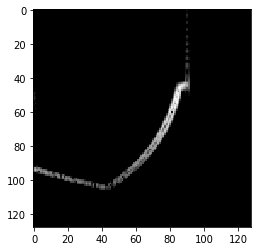
\includegraphics[width=0.3\linewidth]{images/specplot.png}
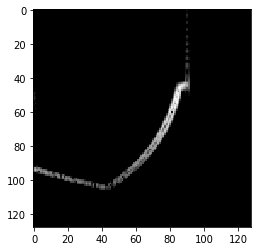
\includegraphics[width=0.3\linewidth]{images/specplot.png}
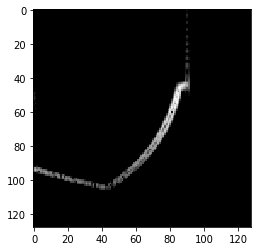
\includegraphics[width=0.3\linewidth]{images/specplot.png}
\caption{1 stack}\label{fig:1stack}
\setcounter{subfigure}{2}%
\end{subfigure}
\caption{Examples of mel-spectrum representations of randomly generated samples. Bigger stacks give us more complex signals, but we find that even stacks of size 1 can be powerful with the right parameters. \colorbox{green!=40}{update this with actual spectrums}}
\label{fig:stackspectrums}
\end{figure}

\subsection{The Ear}
We defined an ear as any method of evaluating a piece of audio, capable of "listening" to a piece of audio and giving it a score (or a list of scores) based on how well it satisfies certain criteria. Since in this work we are mainly focused on percussive generation, what we require from the ear is to give us probabilities of an audio sample belonging to various sound (drum and none-drum) categories. As our synthesizer outputs are deterministic for all programs, allowing us to associate the categorical probabilities of each sound with the program that generated it; navigating our synthesis towards parameters which give us the desired sonic output.\\
%  The most basic representation of a piece of digital audio is via list of numbers and a sampling-rate. For simplicity, we fix the sampling rate to 41,000 per second across all components of this project. An array representation of audio is the representation of the audio within the time domain. More commonly, the frequency domain is used for MIR tasks.
We have implemented several methods of feature extraction and successfully separated different drum categories in interesting ways. 
\todo[inline, color=green!30]{is this the right place to show off some t-sne graphs of how various feature extraction methods separated drum categories? Or take the probability vector assigned to samples by the ear and t-sne that? it might be a cool way to visualize show how well the ear is performing}
A common pitfall of most feature extraction methods implemented is that they do not consider the temporal trends within the audio, making them highly susceptible to errors when evaluating audio that should not belong to any of the categories.\\
Analysis of the frequency content of a piece of audio using windowing functions is a common MIR procedure. Care must be taking such that information critical to percussion categorization such as envelope and temporal changes are not lost in this process. For example, we do not want a reversed kick sample to be labeled as a kick, or even a drum, even if it has the correct frequency content. There are two interconnected temporal trends to consider: 
\begin{itemize}
    \item Change in amplitude within each frequency bin. Harder to measure and utilize and possibly not as important for our purposes, considering the short length of our samples.
    \item Overall amplitude change within a sample. Closely linked to ADSR\\. 
\end{itemize}{}
Temporal trends may be deduced from a spectrum representation of sound. A convolution net trained on our drum dataset, combined with an algorithm ADSR extraction algorithm led to an ear which can reliably reject junk data and samples with inappropriate wave-shapes. \todo[inline,color=green!30]{This paragraph is lying, I haven't done the ADSR algorithm part yet. Highest priority after writing this paper.}
\begin{figure}[H]
\centering
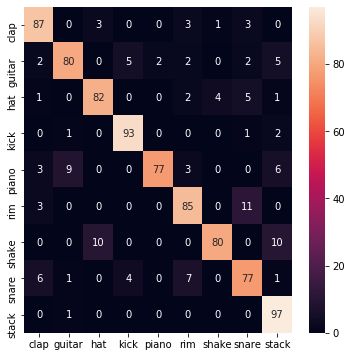
\includegraphics[width=0.8\linewidth]{images/cnn_ear.png}
\caption{confusion matrix of the model working well on a test set. \colorbox{green!=30}{will be updated with new ear.}}
\label{fig:ok ear}
\end{figure}
\todo[inline,color=green!30]{ will add f-measure calculations and other confidence inducing graphs (for example I have a grid of spectrums with the ear's guess vs the actual label under each spectrum, I can colorize the grid depending on whether the guess was correct or not). Code in the notebooks. After updating ear, I will make them look presentable and add them.}
%
% How Can The Synth and Ear Interact?
%
\begin{figure}[H]
\centering
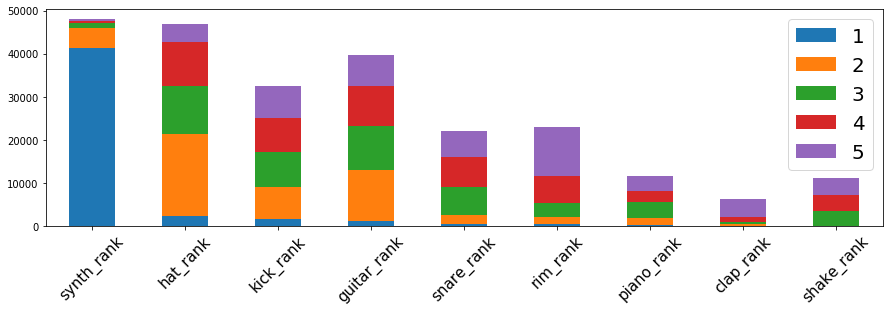
\includegraphics[width=1\linewidth]{images/random_ranks.png}
\caption{\colorbox{green!=40}{labels bigger + show other stack sizes} Showing proportions of categorical ranks for around 50,000 randomly generated sounds. Only showing ranks 1-5. About 90\% received the rank of 1 (blue portion of the bar) for the "synth" category, meaning that the ear correctly gave the highest probability to the sound being from a synth combination. We are interested in the small percentages of random generations that trick the ear due to coincidentally being similar to actual drums (i.e those who received a rank of 1) }
\todo[inline, color=blue!30]{When looking for the best sounds of each category, could use ranks 2 and 3 etc. as well, however:
\unexpanded{\unexpanded{
\begin{itemize}
    \item We must figure out how to penalize their parameters
    \item The task requires even more confidence in ear,
\end{itemize} 
}}} 


\label{fig:rank portions}
\end{figure}
\subsection{How Can The Synth and Ear Interact?}

\begin{figure*}[htbp]
	\centering
		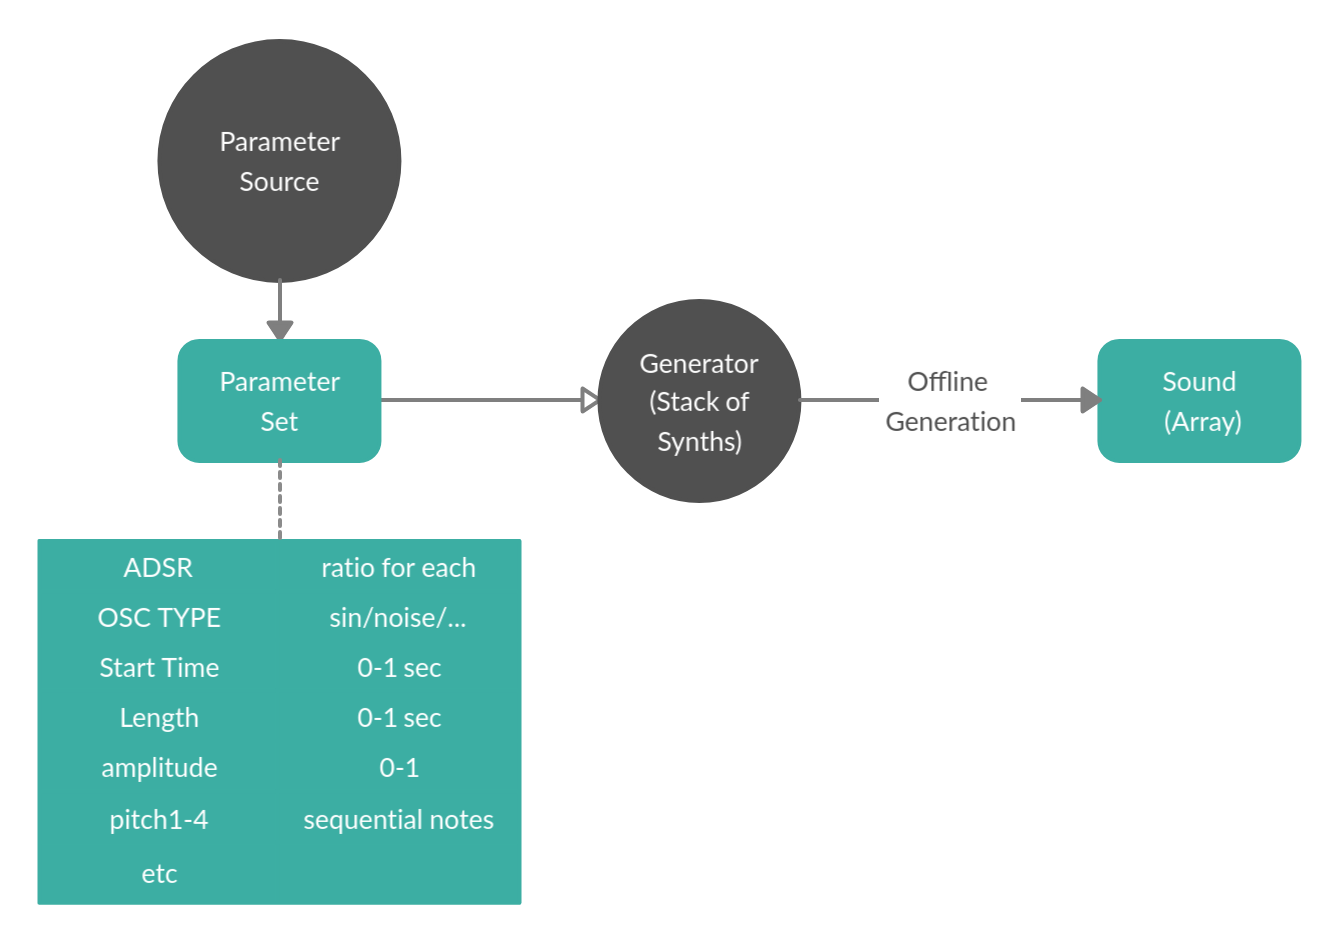
\includegraphics[width=0.7\textwidth]{images/SSS_gen.png}
	\caption{\colorbox{green!=40}{ This graph is bad in many ways.} but would it be worthwhile to have a \textbf{good} flowchart of 
	the generation pipeline in the paper? }
	\label{fig:BlockDiagram2}
\end{figure*}
\label{fig:generation}

With our Synth and Ear in place, we can quickly generate programs for our Synth, create the corresponding audio sample and get the scores for the audio sample. If the ear returns a vector of categorical probabilities, we can assign categorical ranks to the audio sample. For example, the category with the highest probability will have the rank of 1, second highest would rank 2nd, and the lowest probability will have the rank of n (assuming n categories).\textbf{
But how can we use this to create percussion sounds?}\\\\
We utilize our tools in three different methods of generation, with their specific imlpementation discussed in section \ref{gens}.
\begin {enumerate} [label=(\roman*)]
\item Random Generation: We randomly create a drum programs until a sound belonging to our category is produced. We hypothesize that due to the speed of our experiments, it is a viable approach.
\item Multivariate Distribution Sampling: We attempt to learn the joint distribution of our parameters in order to maximize generation of a certain drum category. 
\item Genetic Search: We treat our parameters as genes and attempt to use evolutionary search algorithms to find programs that the ear deems most fit.\\
\end {enumerate} 
\todo[inline,color=blue!30]{As seen in Figure \ref{fig:rank portions}, there is a bias in random generation towards making higher ranking hats and kicks and lower ranking shakers, claps. Is this bias because of Synth structure or a problem with the ear? Will analyse further after updating ear}

\section{Novel Generations}
\label{gens}
\subsection{The Goal}
 Given a category, our aim is to use random generations to guide an algorithm towards novel generation of drums for that category. We evaluate each method by measuring how many samples of categories \textit{kick,snare} and \textit{hat} can be produced in under a minute. Finally we show results of a survey conducted to measure the quality of these samples. 
\subsection{General Methods}
\colorbox{green!=30}{The next 3 sections will be modified heavily after the ear is updated.}
\subsubsection{Random Generation}
To establish a benchmark, we seek to establish the likelihood of generating samples of each category if we generate programs for various stack sizes by random selection of parameters. We have observed a bias in generations as indicated in figure \ref{gens}.\\
\begin{figure}[H]
\centering
\begin{subfigure}[b]{\linewidth}
\includegraphics[width=0.48\linewidth]{example-image-a}
\includegraphics[width=0.48\linewidth]{example-image-a}
\label{fig:1stack}
\setcounter{subfigure}{2}%
\end{subfigure}
\caption{\colorbox{green!=40}{todo}Graphs showing the effectiveness of this method for producing chosesn categories in under a minute}
\label{fig:rand-graphs}
\end{figure}
\subsubsection{Multivariate Distribution Sampling}
\colorbox{green!=40}{go over the math quick}\\
\colorbox{green!=40}{add some graphs showing learned params}\\
\colorbox{green!=40}{add graphs of learned parameters showing why it's not perfect}\\
This method is extremely fast and scalable once the parameter space is calculated. But success is limited due to well known issues with this approach. Notably that the parameter space for virtual synthesizers are often neither differentiable nor Gaussian. \cite{esling2019universal} (a couple more papers also talked about this, \colorbox{green!=40}{I have to look them up}). Currently our parameters are array indices mapping to different values for Synth components. This makes the assumption that our discrete parameter space is normally distributed or differentiable in-appropriate and prone to errors. \\
\begin{figure}[H]
\centering
\begin{subfigure}[b]{\linewidth}
\includegraphics[width=0.48\linewidth]{example-image-b}
\includegraphics[width=0.48\linewidth]{example-image-b}
\label{fig:1stack}
\setcounter{subfigure}{2}%
\end{subfigure}
\caption{\colorbox{green!=40}{todo}Graphs showing the effectiveness of this method for producing chosen categories in under a minute}
\label{fig:multi-graphs}
\end{figure}

\subsubsection{Evolutionary Search}
We implemented evolutionary search using DEAP \citep{DEAP_JMLR2012}. A parameter set is assumed to be an individual with each parameter being its genes. To measure an individuals fitness, we use the formula $fitness=score-rank$. As generations evolve, a Hall-of-Fame list with a fixed size tracks the best individuals to ever live in any given generation, updating itself after each batch of off-springs is evaluated.\\
To ensure diversity of the HOF individuals, the fitness score should also consider some measure of uniqueness. A weighted minkowski distance \footnote{https://docs.scipy.org/doc/scipy/reference/generated/scipy.spatial.distance.minkowski.html} between the genes of an offspring and the HOF individuals may be a good measurement.\\
A generation of $N$ individuals are initialized(randomly or using already existing ranked parameters). To create the offspring generation, each generation goes through mutations and in-place gene crossovers. The new generation consists of the top 80\% of the offspring generation and 20\% new individuals to quicken gene diversity. If the new individuals are coming directly from previously measured high scoring parameter sets, we ensure that they cannot be directly added to HOF without going through mutations and crossovers first.\\

\begin{figure}[H]
\centering
\begin{subfigure}[b]{\linewidth}
\includegraphics[width=0.48\linewidth]{example-image-c}
\includegraphics[width=0.48\linewidth]{example-image-c}
\label{fig:1stack}
\setcounter{subfigure}{2}%
\end{subfigure}
\caption{\colorbox{green!=40}{todo}Graphs showing the effectiveness of this method for producing chosesn categories in under a minute}
\label{fig:evo-graphs}
\end{figure}
\subsubsection{Survey of Generated Drums}
\label{survey}
\colorbox{green!=30}{Finalize ear,generate,make survey.} The survey will be sent out. I know a few producers who are willing to do this.
3 algorithms, 3 categories, 10 samples for each algorithm and category pair, 2 seconds to listen to each sample-> 3 minutes for listening\\
With those numbers I imagine survey will be around 5-6 minutes long.
\subsubsection{Contrasting Ear Scores With Survey Results}
\colorbox{green!=30}{pending section \ref{survey}}

\section{Summary and Conclusions}
\colorbox{green!=30}{Points I want to make:}
\begin{itemize}
    \item Our methodology was successful in generating novel examples of some percussion categories.
    \item Reiterate the importance of ear.
    \item There are potential benefits (e.g: pedagogical, software engineering, efficiency, data search, generality of solution, etc.) to separate some audio generation tasks into multiple parts, rather than throwing everything at some neural net. 
    \item With the right implementation of DSP methods to create a synth, Genetic search (viewed as too slow by previous work) is viable for finding  desired programs and parameters.
    \item Neural nets are function approximators. You don't need them if the actual function is understandable and simple...(but is our task simple enough? how do I prove it?)
    \item When possible, using DSP methods instead of NNs is preferable in many ways(speed,computation,hardware requirements).\\
    \colorbox{green!=30}{Include some speed measurements in appendix?}
    \item ...
\end{itemize}
\section{Future Work}
\colorbox{blue!=30}{Need to think about this more}
\begin{itemize}
    \item Potential for other generative methods (e.g reinforcement learning)
    \item Making the synth's sound range more diverse while maintaining speed and efficiency
    \item Can our approach be used for VSTs?
\end{itemize}
%ACKNOWLEDGMENTS are optional
\section{Acknowledgments}
This section is optional; it is a location for you
to acknowledge grants, funding, editing assistance and
what have you.  In the present case, for example, the
authors would like to thank Gerald Murray of ACM for
his help in codifying this \textit{Author's Guide}
and the \textbf{.cls} and \textbf{.tex} files that it describes.
\section{Ethical Standards}
To ensure objectivity and transparency in research and to ensure that accepted principles of ethical and professional conduct have been followed, authors should include a section “Ethical Standards” before the References, including (if relevant): information regarding sources of funding, potential conflicts of interest (financial or non-financial), informed consent if the research involved human participants, statement on welfare of animals if the research involved animals.

\appendix
%Appendix A
\section{section A}
In case I need an appendix
\subsection{Example Subsection}
\section{Section B}
The sig-alternate.cls file itself is chock-full of succinct
and helpful comments

%%% Place this com
\bibliographystyle{abbrv}
    \bibliography{nime-references} 
\end{document}
